\cotefile{14}
\scanpage{87}
Relations entre hom. de V.A. et groupes de N.S.

\diagram{\resizebox{\linewidth}{!}{\begin{tikzcd}[ampersand replacement=\&,column sep=small,row sep=large]
C^1(A) \arrow[rr] \arrow[d] \& \& H^2(A)\otimes Q_\ell(1)=H^2(A,Q_\ell(1))=\bigwedge^2 H^1(A)\otimes Q_\ell(1)
 \arrow[d,"{\substack{\text{déduit de l'\unsure{accouplt|accouplement}}\\ H^1(A)\times H^1(A^*)\to Q_\ell(-1)}}" ] \& \\
\operatorname{Hom}(A,A^*) \arrow[rr] \arrow[dr,"{\substack{\text{\unsure{application|injection}}\\\text{\textquotedblleft graphe\textquotedblright\ (pas additive!)}}}"] \& \& \operatorname{Hom}(H^1(A^*),H^1(A)) \arrow[dr] \& \\
\& C^n(A\times A^*) \arrow[rr] \& \& H^{2n}(A\times A^*)\otimes Q_\ell(n)
\end{tikzcd}}}

$(n=\dim A)$

\diagram{\begin{tikzcd}[ampersand replacement=\&]
A \arrow[r,"{\bar u=(\mathrm{id}_A,u)}"] \& A\times A^*
\end{tikzcd}}

\diagram{\resizebox{\linewidth}{!}{\begin{tikzcd}[ampersand replacement=\&,row sep=small]
H^{\unsure{*|\bullet}}(A) \arrow[r,"{\bar u_*}"] \& H^*(A\times A^*)(..) \& H^{\unsure{0|\bullet}}(A) \arrow[r] \& H^{2n}(A\times A^*)(n)\\
\& \& \times \& \times\\
H^*(A) \& H^*(A\times A^*) \arrow[l,"{\deleted{\unsure{u^*}}(\bar u^*)}" ] \& H^{2n}(A) \& H^{2n}(A\times A^*) \arrow[l]\\
\& \& \wr \& \unsure{\wr}\\
\& \& Q_\ell(-n) \& Q_\ell(-n)
\end{tikzcd}}}

\diagram{\begin{tikzcd}[ampersand replacement=\&]
H^1(A) \& H^1(A\times A^*)=H^1(A)\times H^1(A^*) \arrow[l,"{(\mathrm{id}_{H^1(A)},u^1)}"]
\end{tikzcd}}

$\bar u_*(1)$

% archive sheet number: 86
\scanpage{88}
\mspage{- 24 -}
\uline{Preuve} : Soit $G$ un faisceau $C'$-acyclique. Il suffit de montrer que pour tout objet $X$ de $C$,
\[
 \overset{\handwritten{\scriptscriptstyle\vee}}{H}{}^q(C^{\unsure{\wedge|\prime}}/X,\handwritten{\mathscr H}^{0}(u_s(G)))=0
 \qquad q\handwritten{>}0
\]

Il suffit donc de montrer que pour toute famille couvrante $\handwritten{\mathcal U}=(U_i\handwritten{\longrightarrow}X,\ i\handwritten{\in}I)$ dont l'existence est assurée par la condition (\unsure{CNC|CMC}), $H^q(\handwritten{\mathcal U},\handwritten{\mathscr H}^{0}(u_s(G)))=0\quad\handwritten{\forall}\ q\handwritten{>}0$. Mais $u$, étant un foncteur continu, transforme la famille couvrante $\handwritten{\mathcal U}$ en une famille couvrante de $u(X)$ ; et par définition du foncteur image directe, on a l'égalité :
\[
 H^q(\handwritten{\mathcal U},\handwritten{\mathscr H}^{0}(u_s(G))) =
 H^q(u(\handwritten{\mathcal U}),\handwritten{\mathscr H}^{0}(G))
\]
Le faisceau $G$ étant $C'$-acyclique, ces groupes sont nuls pour tout $q\handwritten{>}0$. \unsure{c\textsuperscript{o}q.f.d.|c.q.f.d.}

La notion de faisceau $C$-acyclique n'est pas intrinsèque. Elle ne dépend pas uniquement du topos $C^{\handwritten{\sim}}$ défini par le site $C$, mais aussi du site particulier choisi pour définir le topos $C^{\handwritten{\sim}}$ (3.11). Nous allons maintenant définir une propriété intrinsèque.

\margin{\handwritten{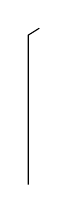
\begin{tikzpicture}[x=1em,y=1em]\draw (0.4,0.25)--(0,0)--(0,-5.4);\end{tikzpicture}}}
\uline{Proposition 3.4} : Soient $E$ un topos annelé par un anneau $A$ de $E$, $F$ un $A$-Module. Les propriétés suivantes sont équivalentes :

\unsure{i|1}) Pour tout objet $S$ de $E$ :
\[
 H^q(S,F)=0 \qquad \handwritten{\forall}\ q\handwritten{>}0\handwritten{.}
\]

\hfill .../...

% archive sheet number: 87
\scanpage{89}
Un homomorphisme $u:A\to B$ de V.A. est connu quand on connaît la classe de cohomologie associée : son graphe dans $A\times B$, \deleted{\unsure{car cela|car cette|en cette} \illegible{1}} (i.e. si on le connaît en tant que \unsure{classe|dans} de corr. cohomologique $l$-adique), car alors on connaît le graphe $\Gamma\inserted{\subset A\times B}$ de $u$ car $T_{Q_\ell}(\Gamma)\subset T_{Q_\ell}(A\times B)$ est alors connu.

\uline{D} $=$, une ss-V.A. de $A$ est connue quand on connaît la classe de cohomologie.

L'\textquotedblleft interprétation\textquotedblright\ cohomologique de l'isom
\[
 C^1(A\times B)/\deleted{\unsure{C^1}} C^1(A)\times C^1(B)\simeq\operatorname{Hom}^{\unsure{\prime}}(A,B^*)
\]
est bien claire, via
\[
\begin{aligned}
&\textstyle\bigwedge^2(H^1(A)\times H^1(B))(1)/\bigwedge^2 H^1(A)(1)\times\bigwedge^2 H^1(B)(1)
 \simeq H^1(A)\otimes H^1(B)(1)\\[-2pt]
&\hfill \rotatebox{90}{$\unsure{\simeq|=|\rotatebox{-90}{$\wr$}}$}\qquad\\[-2pt]
&\hfill \operatorname{Hom}(T_\ell(A),T_\ell(B^*))
\end{aligned}
\]

\uline{Question} Prouver que pour qu'un \unsure{élément|élt|élts} de $H^1(A)\otimes H^1(B)(1)\subset H^2(A\times B)(1)$ soit algébrique

% archive sheet number: 88
\scanpage{90}
\mspage{- 19 -}
\uline{Preuve} : Soit $R$ le crible engendré par les $(U_i\mathrel{\text{---}\!\handwritten{>}}X)$. Le faisceau associé à $R$ est isomorphe au faisceau associé à $X$. On applique alors la proposition précédente et la formule (19).
% A pencil paragraph-break sign precedes « Cette ».
\handwritten{\raisebox{.3ex}{\begin{tikzpicture}[x=.6em,y=.4em]\draw (0,0)--(.7,0)--(.7,1)--(1.6,1);\end{tikzpicture}}}
Cette suite spectrale est \deleted{dûe à} \inserted{\handwritten{celle de}} Cartan-Leray.

\margin{\handwritten{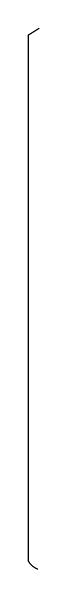
\begin{tikzpicture}[x=1em,y=1em]\draw (.4,.25)--(0,0)--(0,-19) to[bend right=18] (.35,-19.3);\end{tikzpicture}}}
\uline{Corollaire 2.5} : Il existe une suite spectrale fonctorielle en $F$ et en $X$ (objet de $C$) :
\[
 H^{p+q}(C^{\handwritten{\sim}}/X,F)\handwritten{\Longleftarrow}
 \overset{\handwritten{\scriptscriptstyle\vee}}{H}{}^p(X,\handwritten{\mathscr H}^q(F))
\]
Cette suite spectrale fournit, lorsque $X$ varie dans $C$, la suite spectrale de préfaisceaux :
\[
 \handwritten{\mathscr H}^{p+q}(F)\handwritten{\Longleftarrow}
 \handwritten{\check{\mathscr H}}^p(\handwritten{\mathscr H}^q(F))
\]
Ces suites spectrales fournissent des morphismes fonctoriels \handwritten{:}
\margin{\handwritten{$\unsure{\checkmark}$}}
\[
\begin{aligned}
\handwritten{\Phi}^q(F)&:\handwritten{\check{\mathscr H}}^q(\handwritten{\mathscr H}^0(F))\handwritten{\longrightarrow}\handwritten{\mathscr H}^q(F)\\
\handwritten{\Phi}^q_X(F)&:\overset{\handwritten{\scriptscriptstyle\vee}}{H}{}^q(\unsure{E|S}\ X,\handwritten{\mathscr H}^0(F))\handwritten{\longrightarrow}H^q(X,F)
\end{aligned}
\]
Les morphismes $\handwritten{\Phi}^q$ et $\handwritten{\Phi}^q_X$ sont des isomorphismes lorsque $q$ égale $0$ ou $\handwritten{1}$. Les morphismes $\handwritten{\Phi}^2$ et $\handwritten{\Phi}^2_X$ sont des monomorphismes. Plus généralement, lorsque les préfaisceaux $\handwritten{\mathscr H}^i(F)$ sont nuls pour $0\handwritten{<}i\handwritten{<}n$, les morphismes $\handwritten{\Phi}^q(F)$ et $\handwritten{\Phi}^q_X(F)$ sont des isomorphismes pour $0\handwritten{\leq}q\handwritten{\leq}n$ et des monomorphismes pour $q=n+1$.

\uline{Preuve} : La première suite spectrale s'obtient en passant à la limite inductive dans la suite spectrale de la proposition 2.3 sur les

\hfill .../...

% archive sheet number: 89
\scanpage{91}
\begin{flushright}
Tableau des\\
classes de cycles ...
\end{flushright}

% archive sheet number: 90
\scanpage{92}
Anneaux de classes de cycles sur une variété projective non singulière sur un corps $k$ alg. clos

\margin{Autres équivalences : l'équivalence \unsure{régulière} $r$ et les équivalences de Weil wh et $W$ \unsure{définis|définies} par \unsure{Liebermann|Lieberman} .....}

\diagram{\resizebox{.98\linewidth}{!}{\begin{tikzcd}[ampersand replacement=\&,execute at end picture={
\begin{scope}[x=.011cm,y=-.011cm,every node/.style={inner sep=1.5pt}]
\node (num) at (375,90) {$A_{\mathrm{num}}$};
\node (tau) at (375,265) {$A_\tau$};
\node (alg) at (382,525) {$A_{\mathrm{alg}}$};
\node (qh) at (545,255) {$A_{Q_\ell\text{-}\mathrm{hom}}$};
\node (zh) at (545,518) {$A_{\mathbb Z_\ell\text{-}\mathrm{hom}}$};
\node (qhd) at (740,195) {$\deleted{A_{\unsure{Q_\ell|\mathbb Q_\ell}\text{-}\mathrm{hom}}}$};
\node (zhd) at (740,460) {$\deleted{A_{\unsure{Z_\ell|\mathbb Z_\ell}\text{-}\mathrm{hom}}}$};
\node (pic) at (400,865) {$A_{\mathrm{pic}}$};
\node (alb) at (400,995) {$A_{\mathrm{alb}}$};
\node (lin) at (400,1130) {$A_{\mathrm{lin}}$};
\node (gt) at (145,948) {$\unsure{\mathrm{Gr}|G}_{\mathrm{top}} K$};
\node (ga) at (55,1152) {$\mathrm{Gr}_{\mathrm{alg}} K$};
\node (ck) at (208,1340) {$CK$};
\draw[->] (tau)--node[left] {$?\wr$}(num);
\draw[->] (alg)--(tau);
\draw[->] (pic)--(alg);
\draw[->] (alb)--node[right] {$\wr\,?$}(pic);
\draw[->] (lin)--node[right] {$\wr\,?$}(alb);
\draw[->] (ck)--(lin);
\draw[->] (ck)--node[below left] {surj}(ga);
\draw[->] (ga)--(gt);
\draw[->] (lin)--node[below left] {surj}(gt);
\draw[->] (tau)--node[above] {$\overset{?}{\sim}$}(qh);
\draw[->] (alg)--node[above] {$\overset{?}{\sim}$}(zh);
\draw[->] (zh)--(qh);
\draw[->] (qh)--(qhd);
\draw[->] (zh)--(zhd);
\draw[->] (zhd)--(qhd);
\draw[thick] (623,236)--(652,207)--(629,232)--(725,154)--(660,229)--(753,168)--(673,252)--(788,183)--(655,290)--(757,225)--(659,329)--(779,257)--(658,357)--(749,302)--(663,390)--(787,322)--(666,418)--(770,363)--(672,445)--(763,403)--(674,476)--(759,434)--(706,482);
\draw[thick] (557,510)--(580,490)--(566,513)--(611,477)--(586,507)--(646,469)--(621,499)--(677,467)--(652,490)--(700,463);
\draw (295,40)--(642,40)--(642,618)--(314,618)--cycle;
\draw[thin] (642,618)--(916,613);
\draw (324,817)--(610,817)--(623,1190)--(325,1190)--cycle;
\node[anchor=west] (disc) at (810,32) {théorie discrète.};
\draw[->] (disc.west)--(639,82);
\node[anchor=west] (cont) at (667,1132) {théorie continue};
\draw[->] (cont.west)--(619,1126);
\draw[dashed,->] (gt.north east) to[out=-37,in=91] node[pos=.69,above] {$?$} (zh.south);
\draw[->] (gt.north) --(151,516) (151,419) to[out=-90,in=181] (tau.west);
\draw (331,104) .. controls (301,104) and (308,151) .. (292,183) .. controls (284,193) and (283,193) .. (272,196) .. controls (310,201) and (290,262) .. (333,276);
\node[align=center,anchor=east] at (272,210) {groupe libre\\de type fini ?};
\draw (330,286) .. controls (273,294) and (326,413) .. (250,425) .. controls (291,432) and (240,555) .. (340,559);
\node[anchor=east] at (263,456) {Groupe fini ?};
\draw (352,601) .. controls (344,643) and (369,711) .. (306,722) .. controls (360,724) and (342,829) .. (363,837);
\node[anchor=east] at (300,721) {V.A.?};
\node[draw,circle,inner sep=.4pt] (tl) at (482,484) {$\unsure{t\ell|t.C|t.l.}$};
\node[draw,ellipse] (car) at (1015,283) {car. 0};
\draw[thin] (tl)--(car);
\node[align=left,rotate=11,anchor=west] at (952,343) {\unsure{on utilise|ou utiliser|ou meilleure}\\théorie \unsure{infinitésimale|intégrale}.};
\draw (360,1335) .. controls (370,1348) and (435,1334) .. (451,1352) .. controls (456,1336) and (579,1348) .. (584,1334);
\node[align=center,anchor=north] at (481,1364) {flèches toutes\\surjectives};
\draw (49,1438) .. controls (61,1459) and (174,1432) .. (200,1458) .. controls (235,1430) and (354,1458) .. (371,1436);
\node[align=center,anchor=north] at (217,1464) {flèches\\qui sont des\\isom mod torsion};
\end{scope}
}]
{}
\end{tikzcd}}}
% slanted: the connected « car. 0 » note rises to the right.

% archive sheet number: 91
\scanpage{93}
\begin{flushright}
Mumford - Nakai\\
Cycles algébriques\\
amples .....
\end{flushright}

% archive sheet number: 92
\scanpage{94}
\margin{$\nearrow$ N.B. Le critère implique le critère d'amplitude de A. Weil .....}
\uline{Th de Mumford-Nakai} \quad $X$ schéma projectif sur corps $k$, $L$ faisceau inv. sur $X$. Conditions équivalentes :

a) $L$ ample

b) Pour tt \deleted{sous-préschéma fermé intègre $Z$ de $X$} \inserted{faisceau cohérent $F$ sur $X$ \deleted{\unsure{de support}} \unsure{tels que|tel que|tels}} $\dim\operatorname{supp}F\geq1$, on a
\[
 \chi(F\otimes L^{\otimes n})\longrightarrow+\infty\qquad\text{si}\quad n\longrightarrow+\infty
\]

b$'$) Comme b), avec $F$ de la forme $\mathcal O_Z$, $Z$ un sous-préschéma intègre de $X$ de $\dim\geq1$.
\margin{on peut se borner \uline{à supposer}}
% slanted

b$''$) Pour tt sous-préschéma intègre $Z$ de $X$, tel que $\dim Z=1$ (resp. $\dim Z\geq2$) il existe un entier $n=n_Z>0$ tel que $\chi(L^{\otimes n}\otimes\mathcal O_Z)\geq2$ (resp. $\chi(L^{\otimes n}\otimes\mathcal O_Z)\geq1$).

c) Comme b), \uline{en remplaçant $\chi$ par \deleted{$\unsure{h|H^0}$} $\dim H^0$}

c$'$) Comme b$'$)

c$''$) Pour tt sous préschéma intègre $Z$ de $X$ \inserted{tel que $\dim Z=1$ ($\dim Z\geq1$)} existe \unsure{une|un} entier $n=n_Z>0$ tel que $\dim H^0(Z,L^{\otimes n}\otimes\mathcal O_Z)\geq2$ (resp $\geq1$).

\margin{\uline{NB}\quad \uline{Critère numérique} ($X$ irréd de dim $d$) $\left\{\begin{aligned}D.C&>0\quad\text{si }C\text{ courbe irréd }\deleted{\illegible{1}}>0\\D^d&>0\end{aligned}\right.$ (intersection calculée dans $CK(x)$ !)}
% margin note written sideways

\deleted{d) Il existe un entier $n>0$ tel que $L^{\otimes n}$ admette une section \inserted{$\ne0$} ; et pour tout sous-préschéma intègre $Z$ de $X$, \deleted{il existe un} \uline{de dim 1}, il existe un entier $m>0$ tel que $\dim H^0(Z,L^{\otimes\unsure{m|n}}\otimes\mathcal O_Z)\geq2$.}

\deleted{d$'$) \deleted{\unsure{Pour}} Il existe un entier $n>0$ tel que $L^{\otimes n}$ admette une section \inserted{$\ne0$}, et pour tt sous-préschéma intègre $Z$ de $X$, de dim 1, on a $\deg(L\unsure{\otimes\mathcal O_Z|{\mid} Z})>0$.}

% archive sheet number: 93
\scanpage{95}
$\mathrm{a)}\Longrightarrow(\mathrm{b)}+\mathrm{c)})$ bien connu (on peut supposer $L$ très ample, et on applique la théorie du pol. de Hilbert)

\[
\begin{aligned}
\mathrm{b)}&\unsure{\longrightarrow|\Longrightarrow}\mathrm{b}')\Longrightarrow\mathrm{b}'')\quad\text{trivial}\\
\mathrm{c)}&\Longrightarrow\mathrm{c}')\Longrightarrow\mathrm{c}'')\quad\text{trivial}
\end{aligned}
\]

On prouve les autres assertions par récurrence sur \deleted{\unsure{b$'$)}} $\dim X=d$, \unsure{tt|tout|cela|c'} est trivial si $d=0$, et bien connu \deleted{\unsure{si}} si $d=1$. Supposons $d\geq2$

$\mathrm{b}'')\Longrightarrow\unsure{\mathrm{c}|\mathrm{d}}'')$ Grâce au

\uline{Lemme 1} \unsure{Si|Si on} les \deleted{conditions b$''$), $\exists$ \unsure{un} $n_0>0$} \inserted{restrictions de $\underline L$ aux sous préschémas \inserted{intègres}} $Z$ de $X$ de $\dim<d$ sont amples, alors $\exists\,n_0$ tel que
\[
 n\geq n_0\Longrightarrow H^i(X,L^{\otimes n})=0\qquad\text{pour }i\geq2\quad\deleted{\text{\unsure{les supp.}}}
\]
\margin{\unsure{par|pour} des restrictions sur $d=\dim X$ Mais il faut supposer $X$ \unsure{projective|projectiv|projectif}.}
% slanted

cf lettre de Mumford.

\deleted{$\mathrm{d)}\Longrightarrow\mathrm{c)}$ trivial}

\deleted{$\mathrm{d)}\Longrightarrow\mathrm{d}')$ d'après le cas déjà \deleted{\unsure{traité}} \inserted{connu} $d=1$.}

$\unsure{\mathrm{c}|\mathrm{d}}'')\Longrightarrow\mathrm{a)}$ On peut supposer (via : EGA III ... que $X$ est intègre. \deleted{\illegible{1}} \deleted{\unsure{Soit}} \deleted{\unsure{f}} $f$ une section de $L^{\otimes n}$, \deleted{\unsure{A}} $D$ \unsure{l'ens|l'un|l'ens.} de ses zéros, alors $D\ne\varnothing$ car $\underline L$ n'est pas trivial, donc $\dim D=d-1$. On prouve

\uline{Lemme} 2 Sous les conditions du lemme 1, supposons que \inserted{$\exists\,n>0$ tel} $\underline L^{\otimes n}$ ait une section. Alors \deleted{$\unsure{\exists}$} $\exists n_0$ tel que $n\geq n_0\Longrightarrow X\overset{!}{\longrightarrow}\mathbb P H^0(X,L^{\otimes n})$ partout définie et non \unsure{constante|const.|constant}

\margin{$d\geq2$}

cf lettre Mumford ....

\uline{Questions} Dans \unsure{les} énoncés d) et d$'$) peut-on supprimer l'hyp d'existence d'une section $\ne0$ ?? \deleted{\unsure{Oui si} \illegible{2}} \deleted{\illegible{1}} Peut-on supprimer l'hyp. que $X$ projectif ??

% archive sheet number: 94
\scanpage{96}
\diagram{\begin{tikzcd}[ampersand replacement=\&,column sep=small,row sep=tiny]
\overset{\circ}{P}{}^{\unsure{\#|+}}\&\subset\&P^\#\&\subset\&\overline{P^\#}\\
\cup\&\&\&\&\cup\\
\overset{\circ}{Q}{}^\#\&\subset\&Q^+\&=\&\overline{Q^\#}\\
\cup\&\&\&\&\cup\\
\overset{\circ}{\overline R}\&=\&R\&\subset\&\overline R
\end{tikzcd}}

\[
 \boxed{\overset{\circ}{Q}{}^\#\subset P^\#}\qquad\text{d'où}\quad Q^\#=\overline{Q^\#}\subset\overline{P^\#}
\]
\margin{\uline{Prop} de \uline{\unsure{Groth|Groth.}}}
\[
 (\text{donc}\quad \overset{\circ}{Q}{}^\#\subset\overset{\circ}{\overline{P^\#}}=\overset{\circ}{P}{}^\#)
\]
d'où par polarité, comme $Q^+=Q^{+\circ}$
\[
 \overline{P^\#}{}^\circ=P^{\#\circ}\subset Q^\#
\]

\[
 P^+\ni x\Longleftrightarrow \exists\ C>0,\ \inserted{n>0}\ \text{tel que}\quad\gamma(C)=nx
 \Longleftrightarrow
 \boxed{\begin{gathered}\deleted{\text{\unsure{(si $x$ a lieu)}}}\\ \ell(nx)\geq2\ \text{si}\\ n\ \text{grand}\end{gathered}}
\]
\[
 Q^+\ni x\Longleftrightarrow
 \left\{\begin{aligned}x^2&\geq0\\x.a&\geq0\end{aligned}\right.,
 \qquad\overset{\circ}{Q}{}^\#\ni x\Longleftrightarrow x^2>0,\ x.a\geq0
\]
[$a$ choisi dans $\deleted{\unsure{R}}Q^\#$ \unsure{,} p.ex $a$ dans $R$]
\[
 R\ni x\Longleftrightarrow\exists\ C\ \text{\uline{ample}},\ n>0,\ \text{tel que}\quad\gamma(C)=nx
\]

\[
 \boxed{x\in R\ \underset{\substack{\text{th. de}\\\text{Nakai}}}{\Longleftrightarrow}\ \deleted{\unsure{x.P}}\quad x.P>0\quad\text{et}\quad x^2>0}
\]
\figure{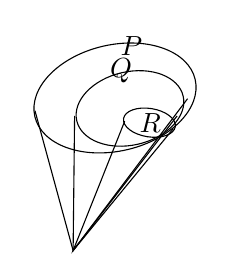
\begin{tikzpicture}[x=.95cm,y=.95cm]
\draw[rotate around={13:(0,1.7)}] (0,1.7) ellipse (1.10 and .71);
\draw[rotate around={13:(.20,1.56)}] (.20,1.56) ellipse (.73 and .49);
\draw[rotate around={-9:(.46,1.37)}] (.46,1.37) ellipse (.35 and .19);
\draw (-1.07,1.53)--(-.56,-.34)--(.97,1.69);
\draw (-.54,1.46)--(-.56,-.34)--(.83,1.46);
\draw (.13,1.39)--(-.56,-.34)--(.78,1.29);
\node at (.22,2.39) {$P$}; \node at (.08,2.07) {$Q$}; \node at (.47,1.37) {$R$};
\end{tikzpicture}}

\[
 \overline R\subset\deleted{\unsure{\bar{\phantom P}}}P^\circ\cap Q=P^\circ=\overline P{}^\circ,\quad\deleted{\unsure{a}}\quad\text{d'où}
\]
\[
 \deleted{\boxed{R\subset\unsure{P|\overset{\circ}{P}}}\quad\unsure{\text{donc}}\ P^\circ}
\]
\[
 R=\overset{\circ}{\overline R}\subset\overset{\circ}{\overline{P^\circ}},
 \qquad\text{je dis qu'on \uline{a égalité}, car}
\]
\[
 \overset{\circ}{P^\circ}\subset\overset{\circ}{Q}\quad\text{et on applique le critère de Nakai}
\]
\[
 \boxed{\begin{aligned}
 R&=\overset{\circ}{\overline{\unsure{R|K}}}=\overset{\circ}{\overline{P^\circ}}\subset\overset{\circ}{Q}\\
 \overline R&=P^\circ=\overline P{}^\circ\subset Q
 \end{aligned}}
\]

\uline{Question} \quad $xP>0\overset{?}{\Longrightarrow}x\in R$

Par Nakai, il reste à voir si $\underline{x^2>0}$ \unsure{Donc|Donné} $x^{\unsure{2}}\geq0$, il \unsure{reste} : voir $x^2\ne0$ On peut supposer que $x$ provient de $D$ div. tel que $D^2=0$. Mais alors $\chi(L(nD))=\chi(X)+n\chi(D)$ et $h^0(L(nD))\geq\chi(L(\unsure{n|m}D))$ pour $n$ grand par Mumford, on doit donc avoir $\chi(D)\unsure{<|\leq}0$

% archive sheet number: 95
\scanpage{97}
Soit $u'$ le composé \deleted{$\unsure{u'_{j,n}|u'_{j,h}}$} $B\quad E_{k,n}\qquad E'_{j,n}\quad u'_{j,h}\quad D'$, où la première flêche est l'hom de transition, alors $u'$ est le relèvement cherché.

\margin{\handwritten{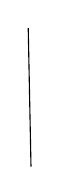
\begin{tikzpicture}[x=1em,y=1em]\draw (0,0)--(.1,-5);\end{tikzpicture}}}
Mettre le corollaire 2.2. sous forme de l'équivalence de trois conditions (i) $B$ form simple (ii) Condition 1º et 2º (iii) $\hat B$ est isomorphe comme alg top à $\hat B'$, où $B'$ est l'algèbre symmétrique d'un $C$-module projectif, munie de \deleted{\unsure{la}} sa topologie définie par son idéal d'augmentation. La forme (iii) est en effet parfois commode, et est obtenue directement dans la démonstration.

\inserted{\handwritten{(\unsure{i$'$bis|i bis}) Pour tout hom de $B$ dans $B'$ \deleted{une \unsure{Algèbre quotient|Algèbre, quotient} \unsure{de} $D'/J$, \unsure{$J$ d'indice}} considéré comme quotient d'une alg. de polynômes \unsure{tronqués}, \deleted{on peut relever \unsure{en un} \unsure{hom}} \deleted{$C[\unsure{t}]$} $B'_{\unsure{(1)|(i)}}$ où $B'_{(0)}=C$, on peut relever,}}
\margin{\handwritten{$\unsure{\text{si}|b'}\ I/I^{\unsure{2|?}}$ de type fini}}
% Left-pointing leader to the small note.

Dans la suite du paragraphe Cohen, 3.4. devient un corollaire immédiat de 3.3. grâce à 2.2. D'ailleurs 3.3. admet toute une kyrielle de corollaires qui dans ma rédaction étaient dans un odre assez chaotique, je suggère \deleted{\unsure{les|le}} l'ordre suivant:

1º Existence d'un corps de représentants dans un anneau \inserted{local noeth} complet, quand l'extension résiduelle est séparable. (Cf 3.5.)

2º (oublié dans ma rédaction). Soit $A$ anneau local nœth complet. Les conditions suivantes sont équivalentes: (i) $A$ contient un corps (ii) Si $\operatorname{car} k(A)=p\quad0$, alors $pA=0$ (iii) $A$ est isomorphe à un anneau quotient d'un anneau $k\ T_1,\ldots,T_n$ sur un corps $k$. (iv) (Si $A$ est intègre de corps des fractions $K$) $k(A)$ et $K$ ont même caractéristique . On peut se borner à donner (iv) à titre de commentaire (c'est une autre façon d'énoncer (ii) simplement), pour \deleted{\unsure{rappeler|rappelerx}} rappeler l'ancienne terminologie \textquotedblleft cas d'égale caractéristique\textquotedblright. Je suggère que nous ne suivions pas cette terminologie, car il est aussi court de \unsure{dife|dire} \textquotedblleft A contient un corps\textquotedblright, et la terminologie \textquotedblleft égale car\textquotedblright\ est fort ambigue pour des anneaux non intègres, par exemple artiniens.

% archive sheet number: 96
\scanpage{98}
\[
 H^2\bigl(L^{\otimes n}\otimes K^{\unsure{\otimes|\otimes\! -}(2n-1)}\bigr)
\]
\noindent\rule{.36\linewidth}{.35pt}

\diagram{\begin{tikzcd}[ampersand replacement=\&,column sep=small,row sep=small]
 \deleted{\unsure{D^d|D^2}} \& \boxed{\left\{\begin{aligned}D^d&>0\\D^{\deleted{\unsure{d-1|n}}}\mathbin{.}C&>0\qquad\text{si}\quad C>0\end{aligned}\right.}\\
 \Updownarrow \& \boxed{\underbrace{D\in P_1^{+\circ}},\quad \alpha_{d-1}D^{d-1}\in P_1^+}\arrow[dr,Rightarrow,start anchor=south west,"\text{\unsure{hyp. de réc|hyp. de vic}}"']\\
 \& \& \deleted{\unsure{\alpha|(}}D^{d-1}\deleted{\unsure{)|\xi}}\in P_{d-1}^{+\circ}
\end{tikzcd}}
\[
 \uline{\text{Question}}\qquad \alpha_{d-1}\bigl(P_{d-1}^{+\circ}\bigr)\subset P_1^+
\]

\diagram{\fbox{\begin{tikzcd}[ampersand replacement=\&,column sep=small,row sep=small]
 P_i^{+\circ}\subset \unsure{\mathcal A|A}^{i}\arrow[r,"\alpha_i"] \& \mathcal A_{\deleted{\unsure{2|n}}d-i}\supset P_{\deleted{2}d-i}^{+}\\[-1ex]
 \rotatebox{90}{$=$}\hspace{4em}\&\\[-1ex]
 P_+^{\unsure{\circ|2|i}}\hspace{4em}\&\\
 P_{\deleted{2}d-i}^{+\circ}\subset\mathcal A^{2d-i}\arrow[r,"\alpha_{d-i}"]\&\mathcal A_i\supset P_i^+\\
 \operatorname{int}\bigl(P_i^{+\circ}\bigr)\arrow[r]\&P_{\deleted{2}d-i}^{+}
\end{tikzcd}}}
\[
 c_{\unsure{i|1}}^{\unsure{j|i}}(E)
\]
% archive sheet number: 97
\scanpage{99}
$\unsure{0|O}_{\mathrm{IV}}\quad$ \uline{Différentielles et dérivations.}

\deleted{NB} Il nous a paru utile de développer les notions différentielles en utilisant la notion d'algèbre topologique formellement simple,définie dans ``Cohen'' . Dans les premiers numéros qui suivent, nous n'utiliserons que la définition``Cohen''1.1. et éventuellement une partie des sorites \unsure{conténus|contenus} dans 1.2.

NB Il se trouvera donc que cette rédaction \unsure{contient|contint} un bon nombre de résultats de ma rédaction ``Cohen différentiel'', qu'il y aura lieu de \unsure{refondre|refôndre} en conséquence.

1. \uline{Dérivations et extensions d'algèbres}.

\uline{Proposition} 1.1. Soient $A$ un anneau, $B$ une $A$-algèbre, $p:E\quad C$ un homomorphisme de $A$-algèbres dont le noyau $J$ est de carré nul, $u:B\quad C$ un homomorphisme de $A$-algèbres. Supposons qu'on ait un homomorphisme de $A$-algèbres $v_1:A\quad E$ qui relève $u$ i.e. tel que $pv_1=u$. Pour qu'une application $v_2:B\quad E$ ait la même propriété, il f et s qu'on ait
\[
 v_2-v_1=D\quad\text{i.e.}\quad v_2=v_1+D
\]
où $D:B\quad J$ est un application satisfaisant les deux conditions suivantes: 1º $D$ est $A$-linéaire 2º pour $f,g\quad B$, on a $D(fg)=fDg+D(f)g$

On notera que compte tenu de 2º), 1º) équivaut aussi à \deleted{1 bis}

1 bis) $D$ s'annule sur $\operatorname{Im}(A\quad B)$.

\uline{Définition} 1.2. D'une dérivation d'un anneau dans \unsure{un|uh} module, d'une $A$-dérivation d'une $A$-algèbre $B$ dans un $B$-module $J$.

\uline{Corollaire} 1.3. Etant donnés $A,B$, \deleted{$E$,} $p:E\quad C,J$, $u:B\quad C$ comme dans 1.1. \deleted{\unsure{L'ensemble pour tout relèvement|l'ensemble pour tout relèvement}} l'ensemble des relèvements de $u$ en un homomorphisme $v$ de $A$-algèbres est vide, ou un ensemble principal homogène sous l'action du groupe $\operatorname{Dér}_A(B,J)$
% archive sheet number: 98
\scanpage{100}
\diagram{\begin{tikzcd}[ampersand replacement=\&,row sep=small]
 D^{\deleted{\unsure{i|1}}}\mathbin{.}C\geq0\qquad\text{si}\qquad C>0\arrow[d,Rightarrow,"?"]\\
 D^iX_i\geq0\qquad\text{si}\qquad X_i>0\qquad ??
\end{tikzcd}}
\[
 D^{\deleted{\unsure{1|i}}}\in P_1^{+\circ}\Longrightarrow D^i\in P_i^{+\circ}
 \qquad\text{pour}\quad i\leq d-1\qquad\uline{\text{hyp. de réc.}}
\]
\[
 \deleted{\unsure{D^2|D^d}}\qquad\text{\unsure{aura-t-on}}\qquad
 D^d\in P_d^{+\circ}\quad\text{i.e.}\quad D^d\geq0\quad ??
\]
\[
 \text{On a}\qquad D^d =
 \underset{\substack{\rotatebox{-90}{$\in$}\\P_i^{+\circ}}}{D^i}
 \underset{\substack{\rotatebox{-90}{$\in$}\\P_{d-i}^{+\circ}}}{D^{d-i}}
 \qquad (0<i<d)
\]

\diagram{\begin{tikzcd}[ampersand replacement=\&,row sep=small,column sep=small]
 \boxed{P_i^{+\circ}\mathbin{.}P_{d-i}^{+\circ}\geq0\quad ?}\arrow[d,Leftrightarrow] \&
 P_i^{+\circ}P_j^{+\circ}\subset P_{\unsure{i\mathrm e j|i+j}}^{+\circ}\arrow[l,Rightarrow]\\
 \boxed{\alpha_i(P_i^{+\circ})\subset P_{d-i}^+}\arrow[d,Leftrightarrow]\&\\
 \boxed{\alpha_{d-i}(P_{d-i}^{+\circ})\subset P_i^+}\&
\end{tikzcd}}

\diagram{\begin{tikzcd}[ampersand replacement=\&,row sep=small]
 D\mathbin{.} C\geq0\qquad\text{si }C\geq0\\
 D^2\mathbin{.}\deleted{\unsure{D_i|D}}\mathbin{.}D'\geq0\qquad\text{si }D'\geq0\arrow[d,Rightarrow,"?"]\\
 D^3\geq0
\end{tikzcd}}
\figure{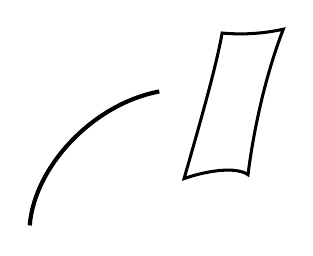
\begin{tikzpicture}[x=.70cm,y=.70cm]
 \draw[line width=1.5pt] (0,0) .. controls (.08,1.05) and (1.13,2.20) .. (2.35,2.43);
 \draw[line width=1.1pt] (2.80,.85) .. controls (3.05,1.72) and (3.38,2.86) .. (3.49,3.49)
 .. controls (3.83,3.46) and (4.19,3.47) .. (4.60,3.56)
 .. controls (4.24,2.63) and (4.04,1.58) .. (3.96,.92)
 .. controls (3.75,1.07) and (3.23,1.00) .. cycle;
\end{tikzpicture}}
\diagram{\begin{tikzcd}[ampersand replacement=\&]
 P_1^{+\circ}\subset\unsure{\mathcal A|A}^1\arrow[r]\&\mathcal A_2\supset P_2^+
\end{tikzcd}}
\[
 \deleted{\unsure{D+n|D+}}\qquad D'+nD\in P_2^+
\]
\[
 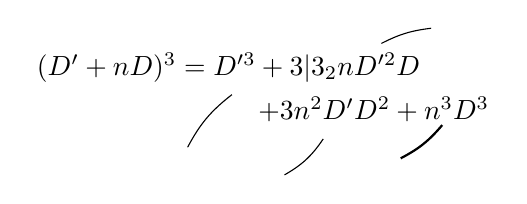
\begin{tikzpicture}[x=1em,y=1em]
 \node[anchor=base west] at (0,1.6) {$(D'+nD)^3=D^{\prime 3}+\unsure{3|3_2}nD^{\prime 2}D$};
 \node[anchor=base west] at (8.0,0) {$+3n^2D'D^2+n^3D^3$};
 \draw (12.8,2.75) to[bend left=10] (14.6,3.3);
 \draw[thin] (5.8,-1.0) to[bend left=12] (7.4,.9);
 \draw[thin] (9.3,-2.0) to[bend right=13] (10.7,-.7);
 \draw[thick] (13.5,-1.4) to[bend right=11] (15,-.2);
 \end{tikzpicture}
\]
\figure{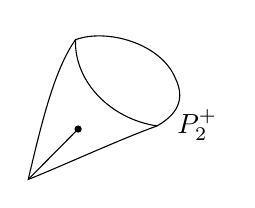
\begin{tikzpicture}[x=.66cm,y=.66cm]
 \draw (.05,0) .. controls (.31,1.10) and (.55,2.11) .. (.96,2.69)
 .. controls (1.57,2.91) and (2.60,2.62) .. (2.88,1.95)
 .. controls (3.14,1.43) and (2.75,1.16) .. (2.53,1.03)
 .. controls (1.83,.78) and (.68,.25) .. cycle;
 \draw (.96,2.69) .. controls (.93,1.88) and (1.64,1.16) .. (2.53,1.03);
 \draw (.05,0)--(1.01,.97); \fill (1.01,.97) circle (.07);
 \node[right] at (2.73,1.05) {$P_2^+$};
\end{tikzpicture}}
\[
 \begin{aligned}
 &\deleted{D+\tfrac1nD'}\\
 &D'+nD\simeq
 \end{aligned}
 \qquad\boxed{D^3\geq0}
\]
% archive sheet number: 99
